\documentclass[12pt]{article}

\usepackage[utf8]{inputenc}
\usepackage{textcomp}
\usepackage{hyperref,xcolor}
\usepackage{graphicx}
\usepackage{qrcode}
\usepackage[scaled]{helvet}
\usepackage[
    type={CC},
    modifier={by-nc-sa},
    version={4.0},
]{doclicense}

\renewcommand\familydefault{\sfdefault}

\newcommand\degree[1]{\mbox{#1 \textdegree{} Cesius}}
\newcommand{\versionsnummer}{1.1-SNAPSHOT} 
\newcommand{\homeurl}{https://github.com/codirk/gelato/releases}

\graphicspath{{images/}}
\DeclareGraphicsExtensions{.pdf,.png,.JPG}


% ##################
% # BEGIN DOCUMENT 
% ##################

\begin{document}

\thispagestyle{empty}

%\abstract{
%	Bei diesem Dokument handelt es sich um eine kleine Zusammenfassung zur Eisbereitung. Die Mengenangaben sind für eine MUSSO-Mini (700 g) optimiert.
%	}

\title{ Gelato }
\author{Dirk Messetat}
\date{\today}


\maketitle

\begin{center}
	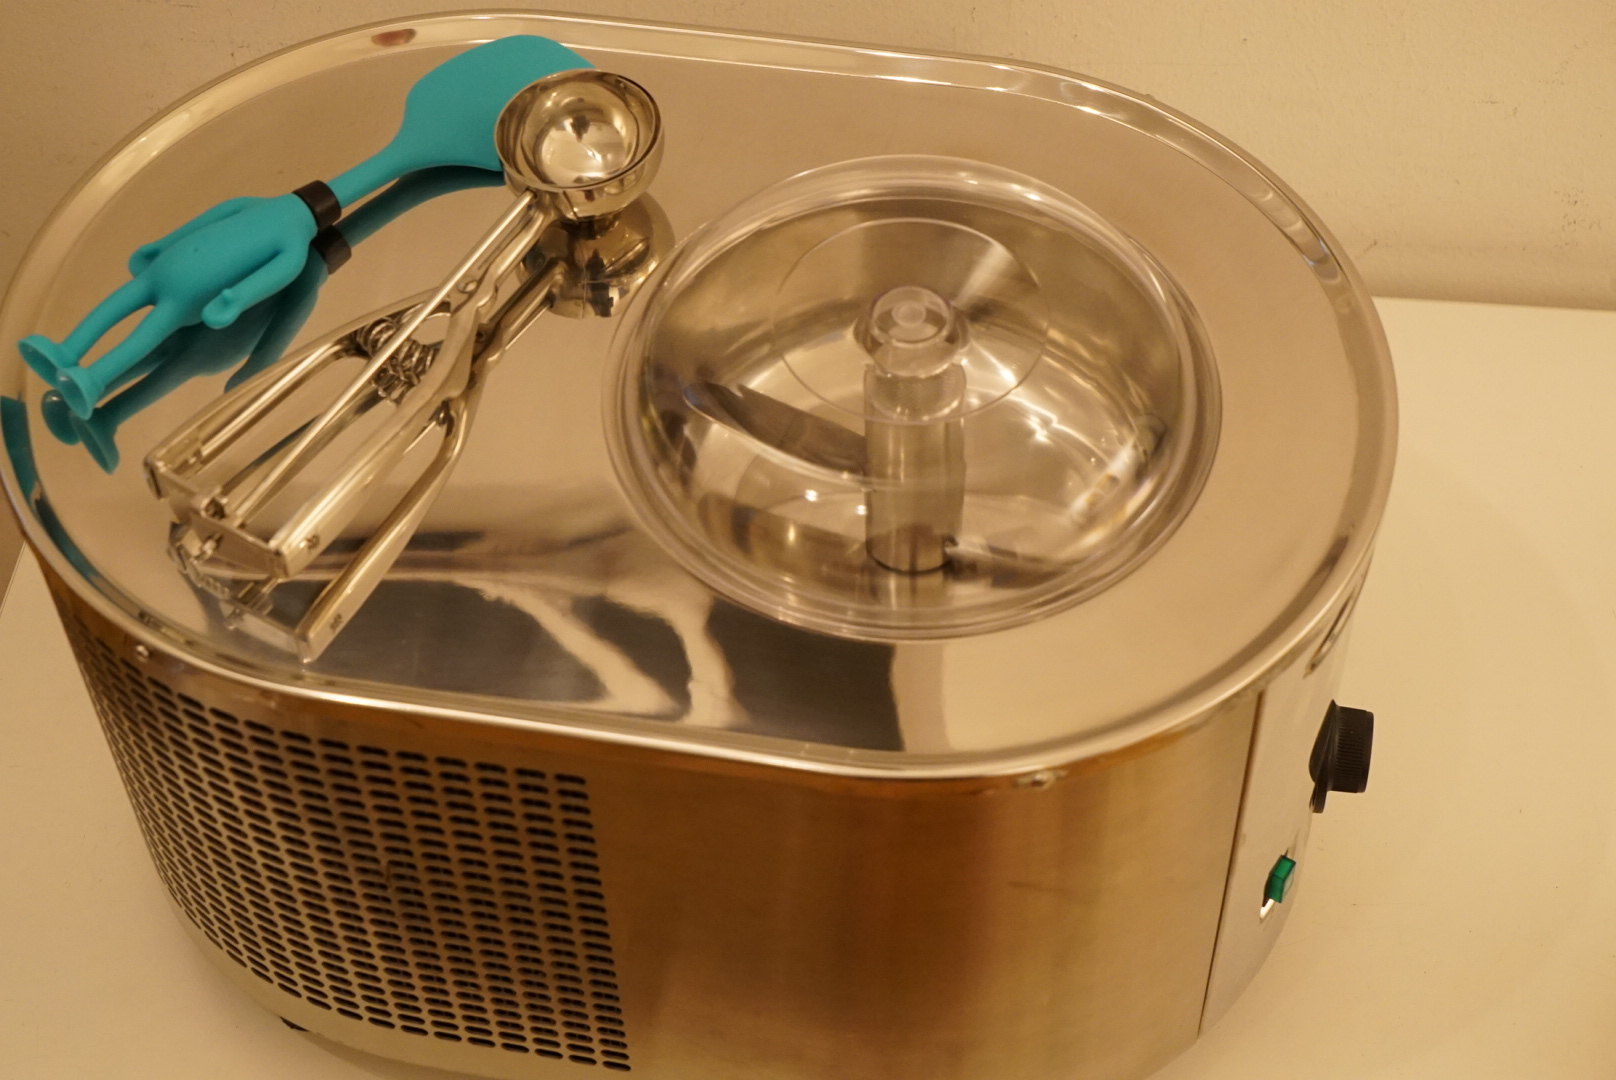
\includegraphics[scale=0.75, angle=0]{DSC07545}
\end{center}


\begin{center}

\small Version: \versionsnummer \\
	\hfill\break
	\qrcode[height=1in]{\homeurl} \\
	\hfill\break
	\texttt{ \url{\homeurl}}

\end{center}

\begin{center}
\doclicenseText
\newline
\newline
\doclicenseImage

\end{center}


\begin{center}
\small{Dieses Dokument wurde mit \LaTeX{} gesetzt.}

\end{center}

\pagebreak

\tableofcontents

\clearpage
\newpage

% ##################
% # BEGIN CONTENT 
% ##################

\part {Einkaufslisten}
\section{Ausstattung}


\begin{itemize}
 	\item \href{https://amzn.to/43WvDjI}{MUSSO Mini Eismaschine}
 	\item \href{https://amzn.to/3U14BmH}{Contacto Zylinder-Form-Dichtung für die MUSSO beim Umfüllen}
	\item \href{https://amzn.to/3w2hKUm}{Feinwage (GRAM PRES Hochpräzise Milligramm-Waage)}	
	\item \href{https://amzn.to/3vR03XR}{Thermometer Löffel (Rosenstein \& Söhne Kochthermometer 3in1-Kochlöffel)}
	\item \href{https://amzn.to/4aTZBH4}{4 x Eisbehälter (SPRINGLANE 4er-Set Eisbehälter für Speiseeis 400ml)}
	\item \href{https://amzn.to/3UiqkIe} {Waffeleisen (Cloer 2898EF Hörncheneisen Professional Ostfrieslandwappen)}
	\item Thermomix TM6
	\item \href{https://amzn.to/3PZtSME}{Norpro Edelstahlschaufel, 39 mm (1,5 Tablespoon)}
	\item Lebensmitteldesinfektion	
\end{itemize}

\newpage
\section{Zutaten}
\subsection{Basiszutaten}
\begin{itemize}
  \item Milch (Berchtesgadener Land Bio 3,5 \%)
  \item Sahne (Berchtesgadener Land Bio)
  \item \href{https://faszination-vanille.de/product/stange-tahiti-vanille/}{\textit{Vanilla Tahitensis}}  (Tahiti-Vanille) oder Zitronenschale
  \item Salz
  \item \href{https://www.feldt-honig.de/bio-honig-500g-glas/61/bio-suessklee-500-g-sardinien/de-oeko-006}{\textit{Süßkleehonig}}
\end{itemize}

\subsection{Zucker}
\begin{itemize}
 	\item Zucker (Naturata Roh-Rohrzucker demeter Bio)
  	\item 500 g Bio Trockenglukose DE33 - DE42
   	\item 500 g Bio Dextrose (Traubenzucker)
  	%\subitem Maltodextrin (Kohlenhydratpulver) - sehr selten benutzt
\end{itemize}

\subsection{Bindemittel}
\begin{itemize}
	\item Eier oder
	\item Bindemittelmischung
	   \begin{itemize}
			\item 250 g Bio Guarkernmehl (E412)
			\item 250 g Bio Johannisbrotkernmehl (E410)
			\item 250 g Bio Inulin (keine E-Nummer)
			\item 125 g Bio Pektin (E440 / bei Warmzubereitung)
			%\item Lecithin
		\end{itemize}		
\end{itemize}
\subsection{Trockenpulver}
\begin{itemize}
	\item Magermilchpulver
	\item Joghurtpulver
\end{itemize}


\subsection{Frostschutz}
\begin{itemize}
  	\item Pflanzliches Glycerin (E422) - Lebensmittel-/Pharmaqualität 95\%
\end{itemize}

\subsection{Kuvertüre}
\begin{itemize}
	\item Kuvertüre Callets
	\begin{itemize}
  		\item Callebaut 70-30-38
  		\item Callebaut Receipe RB1 - Pinke Schokolade
  		\item Callebaut Receipe No. W2 - Weiße Schokolade
	\end{itemize}
\end{itemize}


\newpage
\part{Allgemein}

\section{Zubereitung Eismasse (Thermomix TM6)}
	\begin{enumerate}
		\item Zutaten hinzufügen
		\item ggf. Stange Vanille aufschneiden, auskratzen und hinzugeben
		\item 12 Min./85°C/Stufe 2
		\item Im Anschluss für 2 Stunden ins Eisfach.
\end{enumerate}


\section{Zubereitung Eismasse (Klassisch)}
	Für alle die grad keinen Thermomix TM6 zur Hand haben, oder einfach den gesamten Schaffensprozess zelebrieren möchten.
	\begin{enumerate}
  		\item Die Eidotter mit dem Zucker zu einer schaumigen Creme verrühren.
  		\item In einen flachen Topf die Milch und die Sahne erwärmen und die Zitronenschale (oder die Vanilleschote) zur Aromatisierung hinzugeben.
  		\item Die Eidotter-Creme in die erwärmte Milch geben und auf max. \degree{85} im Wasserbad erhitzen (zur Rose lassen).
  		\item Abkühlen lassen (am besten auch ein paar Stunden im Kühlschrank ruhen lassen), dann die Zitronenschale bzw. Vanilleschote herausnehmen und das Gemisch in den Speiseeiszubereiter geben.
	\end{enumerate}


\section {Glycerin}
Damit das Eis nicht knochenhart im Eisfach mit \degree{-18} wird.

Das Glycerin wird erst in die Eismaschine gegeben, wenn das Eis bereits eine gewisse Konsistenz erreicht hat (50\% der Gesamtdauer), weil es sonst auch nicht in der Eismaschine gefrieren wird.

Es sollte mindestens 10-20 ml Glycerin auf 700 g Eismasse verwenden werden. 

\textbf{Wenn das Eis Alkohol enthält wird kein Glycerin hinzugefügt. }


\section{Zubereitung in der Eismaschine}
Das Eis hat die richtige Konsistenz erreicht, wenn die Eismasse nicht mehr glänzt also matt ist. 
\begin{itemize}
  \item 1 Eiweiß hinzufügen (optional)
  \item Der Timer sollte auf 20-25 Minuten gestellt werden.
  \item Nach 15 Minuten Glycerin hinzufügen.
  \item Nach 25 Minuten die Kühlung deaktivieren und noch 2 Minuten weiterlaufen lassen.
  \item Mindestens 2 Stunden in das Eisfach
\end{itemize}


\section{Blanchieren wegen Bromelain}
\begin{itemize}
  \item Kiwis, Mangos, Papaja, Ananas
\end{itemize}
Müssen bei \degree{60} blanchiert werden, damit das Bromalein zerstört und die Milch nicht sauer wird.

\newpage
\part{Eis - Rezepte}

\section {Einleitung}
Vom Prinzip her gibt es drei Grundarten von Eis:
\begin{itemize}
  \item Milchspeiseeis (warme Zubereitung)
  \item Milchspeiseeis (kalte Zubereitung) wie Joghurteis/Buttermilcheis/...
  \item Sorbets (kalte Zubereitung)
\end{itemize}

Milchspeiseeis kann mit oder ohne Ei hergestellt werden. Der Vorteil der  Variante ohne Ei ist die Haltbarkeit. Mit Ei ca. 2 Wochen, ohne Ei ca 4-6 Wochen. Je nachdem wie gut das Eis schmeckt, kann die Haltbarkeit signifikant reduziert werden.

Des weiteren sind bei der modernen Variante die Trockenanteile erhöht, um die Gefrierhemmung im Eisfach bei \degree {-18} zu verbessern.



% ####################
% # Creme-Speiseeis
% ####################

\section {Klassisch}

\subsection {Einleitung}
Die folgenden klassischen drei Basisrezepte dienen als Ausgangslage aller Eisrezepte dieses Dokumentes. Sie werden später in der modernen Zubereitungsart dahingehen modifiziert, dass das Eis auch bei \degree{18} noch geschmeidig bleibt.  

\newpage
\subsection {Creme-Speiseeis (klassisch)}
\subsubsection {Zutaten}
\begin{itemize}
  	\item 250 g Milch 
  	\item 250 g Sahne oder Mascarpone
  	\item 125 g Zucker
  	\item 4 - 6 Eigelb % (75 g)
  	\item Vanilleschote oder Zitronenschale
  	\item Prise Salz
\end{itemize}

\subsection {Joghurt-Speiseeis (klassisch)}
\subsubsection {Zutaten}
\begin{itemize}
  \item 300 g Vollmichjoghurt (griechisch)
  \item 250 g Sahne
  \item 150 g Zucker
  \item Saft einer halben Zitrone %(25 g)
  \item Prise Salz
\end{itemize}

\subsection {Sorbet (klassisch)}
\subsubsection {Zutaten}
\begin{itemize}
  	\item 500 g Frucht (z.B. Himbeeren/Flugmango/...)
  	\item 175 g Zucker
  	\item Saft einer halben Limette %(25 g)
  	\item Prise Salz
  	\item 1 TL Raps- oder Sonnenblumenöl (optional) 
\end{itemize}

\pagebreak
\section {Modern}

\subsection{Fertigpulver}

Grundzusammensetzung (Vorrat für eine 1L Dose (565 g)):

\begin{itemize}
  \item 1 (4) g Johannisbrotkernmehl
  \item 1 (4) g Quarkernmehl
  \item 11 (44) g Inulin 
  \item 40 (160) g Trockenglukose
  \item 60 (240) g Dextrose
\end{itemize}


\pagebreak
\subsection {Creme-Speiseeis}

\subsubsection {Zutaten (710 g)}
\begin{itemize}
	\item 80 g \textbf{\textit{Fertigpulver}}
  	\item 1 g Pektin (nur heiß)
  	\item 25 g Magermilchpulver
\end{itemize}
\begin{itemize}
  	\item 250 g Milch 
  	\item 250 g Sahne oder Mascarpone
  	\item 100 g Zucker
  	\item Vanilleschote oder Zitronenschale
  	\item Prise Salz
\end{itemize}

\subsubsection {Zutaten mit Ei (710 g)}

Hier werden vom Creme-Speiseeis 
\begin{itemize}
  \item von 250 g Milch werden 75 g Milch (= 175 g) mit
  \item 4 - 6 Eigelb
\end{itemize}
ersetzt.


\subsubsection {Tips}
	Diese Creme-Speiseeis-Grundlage lässt sich auf vielerlei Arten variieren: 
	\begin{itemize}
  		\item Man kann beispielsweise, kurz bevor die Speiseeismasse ihre endgültige Festigkeit erreicht, grob zerriebene  \href{https://www.lotusbiscoff.com/de-de}{\textit{Lotus Biscoff Kekse}} direkt in den Eisbereiter geben.
  		\item 15 ml Glyzerin.
	\end{itemize}


\pagebreak

\subsection{Erdbeer-Eis}
\subsubsection {Zutaten}
	Hier werden vom Creme-Speiseeis 
	\begin{itemize}
	  \item 150 g Milch / 150 Sahne mit
	  \item 300 g Frucht
	\end{itemize}
	ersetzt:

\begin{itemize}
 	\item 300 g Erdbeeren
\end{itemize}
\begin{itemize}
	\item 80 g \textbf{\textit{Fertigpulver}}
  	\item 1 g Pektin (nur heiß)
  	\item 25 g Magermilchpulver
\end{itemize}
\begin{itemize}
  	\item 75 g Milch 
  	\item 100 g Sahne oder Mascarpone
  	\item 50 g Zucker
  	\item 4 - 6 Eigelb
  	\item Vanilleschote oder Zitronenschale
  	\item Prise Salz
\end{itemize}
\subsubsection {Tips}
Wenn vorhanden 50 g Erdbeeren mit 50 g gefriergetrockneten Erdbeeren ersetzen. 

\subsection{Schokoladen-Eis}
\subsubsection {Zutaten}
	Hier werden vom Creme-Speiseeis 
	\begin{itemize}
	  \item 100 g Zucker mit
	  \item 100 g Callebaut
	\end{itemize}
	ersetzt:
	
	\begin{itemize}
		\item 100 g Callebaut
	\end{itemize}
	\begin{itemize}
		\item 80 g \textbf{\textit{Fertigpulver}}
	  	\item 1 g Pektin (nur heiß)
	  	\item 25 g Magermilchpulver
	\end{itemize}
	\begin{itemize}
	  	\item 200 g Milch 
	  	\item 200 g Sahne oder Mascarpone
	  	\item 30 g Zucker
	  	\item 4 - 6 Eigelb % (75 g)
	  	\item Vanilleschote oder Zitronenschale
	  	\item Prise Salz
	\end{itemize}

\subsubsection{Tips}
\begin{itemize}
	  \item 20 ml Glyzerin.
\end{itemize}

% ####################
% # Joghurt-Eis
% ####################

\pagebreak
\subsection{Joghurt-Eis}

\subsubsection{Zutaten (710 g)}
\begin{itemize}
	\item 80 g \textbf{\textit{Fertigpulver}}
  	\item 20 g Magermilchpulver
  	\item 40 g Joghurtpulver
\end{itemize}
\begin{itemize}
  \item 300 g Vollmichjoghurt (griechisch)
  \item 150 g Sahne
  \item 120 g Zucker
  \item Saft einer halben Zitrone %(25 g)
  \item Prise Salz
\end{itemize}
\subsubsection{Tips}

\begin{itemize}
	  \item Wenn weiße Joghurt-Creme statt Joghurt verwendet, wird das Eis noch cremiger.
	  \item Buttermilch/Kefir/Quark/... sollte ebenfalls funktionieren.
	  \item 150 Kokosmilch statt Sahne ist auch lecker.
	  \item 10 ml Glyzerin.
\end{itemize}


% ####################
% # Sorbet
% ####################

\subsection{Sorbet}
\subsubsection {Zutaten (710 g)}
\begin{itemize}
  	\item 80 g \textbf{\textit{Fertigpulver}}
\end{itemize}
\begin{itemize}
  	\item 450 g Frucht (z.B. Himbeeren)
  	\item 150 g Zucker
  	\item Saft einer halben Limette % (25g)
  	\item Prise Salz
  	\item 1 TL Raps- oder Sonnenblumenöl (optional) 
\end{itemize}


\newpage
\part{Eiswaffeln}
\section {Waffel}
\subsection{Zutaten}
\begin{itemize}
  \item 2 Eier
  \item 175 g Butter
  \item 200 g Zucker
  \item 250 ml Wasser
  \item 2 P. Vanillezucker
  \item 350 g Mehl
\end{itemize}
\subsection{Zubereitung}
\begin{enumerate}
  \item Die 175g Butter  3 Min./60°C/Stufe verflüssigen.
  \item Zucker mit Vanillezucker vermischen, mit der flüssigen Butter, dem Mehl, den Eiern und dem Wasser 3 Min./Stufe 2.5 zu einem glatten Teig verrühren.
  \item Der Teig muss gut vom Löffel fließen. Ist dies nicht der Fall, noch etwas Wasser hinzufügen.
  \item Der Teig muss mindestens 2 Stunden ruhen.
  \item Zum Backen den Teig mit einer kleinen Schöpfkelle in den hinteren Teil der Backform einfüllen, den Deckel schnell schließen, und die Griffe für einige Sekunden fest zusammendrücken.
\end{enumerate}
\subsection{Tips}
\begin{itemize}
  \item Statt der 2 Eier kann einfach das restliche Eiweiß von er Eismasse verwendet werden.
\end{itemize}


\newpage
\part{Eisideen}

\section {Common}
\begin{itemize}
  \item Minz-Eis
  \item Grüntee-Eis
  \item Lemon-Pie-Eis
  \item Karamel-Pekannuss-Eis
  \item Safran-Orangen-Eis mit Mandelkrokant
  \item Lotus-Spekulatius-Creme-Eis
  \item Salz-Karamel-Eis
  \item Süßholz-Anis-Eis
  \item Schneeweiß-Kaffee-Eis
  \item Safran-Walnuss-Eis
  \item Haselnuss-Eis
  \item Gebrannte-Mandeln-Eis
  \item After-Eight-Eis
\end{itemize}

\section {Mit Alkohol}

\begin{itemize} 
  \item Bacio-Eis
  \item Baileys-Eis
  \item Rosinen-Rum-Eis
  \item Caipirinhia-Sorbet
  \item Campari-Oragen-Sorbet
  \item Gin-Tonic-Sorbet
  \item Pina-Colada-Sorbet
\end{itemize}

\section {Spezial}
\begin{itemize}
  \item Parmesan-Eis
  \item Tomaten-Eis
\end{itemize}


\end{document}